\section{Results}
\label{sec:results}

\subsection{Main Accuracy}

Table~\ref{tab:main} summarizes the accuracy progression, and
Figure~\ref{fig:curves}(a) shows the corresponding validation curves. A plain
200-epoch student reaches 94.76\% validation accuracy. Adding the full training
recipe (300 epochs, TrivialAugment, Cutout, mixup/CutMix, SAM, EMA) raises this to
97.36\%, a gain of 2.6 points. Two-teacher KD adds 0.38 points (97.74\%), and a
third teacher adds only 0.02 points (97.76\%), which is within noise. Moving to
the wider \texttt{r3\_80} student and 600 epochs reaches 97.84\% raw and 97.92\%
under 5-crop TTA. Extending to 1,200 epochs changes the holdout number by
$-0.02$ raw and $+0.02$ under 5-crop (97.82/97.94), i.e.\ it is not distinguishable
from 600 epochs on this split.

The full-data models have no unbiased validation score. The public leaderboard
scores are 0.904 for the two-teacher student and 0.911 for the selected
\texttt{F2s1} model (5-crop TTA; 0.903 with flip TTA only). The team's private
score is 0.880, placing 13th. Because both \texttt{F2s1} and the two-teacher
student were selected as final submissions, the private score cannot be
attributed to a single model. Figure~\ref{fig:leaderboard} collects every public
submission; the selected 0.911 and 0.904 are the best two.

A 4.88M student beats the 28.5M PyramidNet teacher (97.64\%) on the holdout, and
comes within 0.3 points of the best teacher pool (98.14\%). This is the expected
effect of distillation with a long schedule and strong augmentation: the student
inherits the ensemble's function while seeing more effective regularization than
any single teacher. Figure~\ref{fig:teachers} compares the teachers and the two
selected students directly.

\begin{figure}[t]
\centering
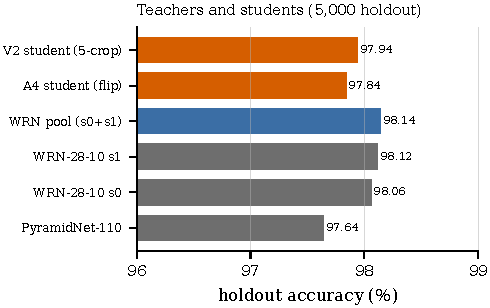
\includegraphics[width=\columnwidth]{figures/fig_teacher_student.pdf}
\caption{Teacher and student holdout accuracy. The 4.88M student is below the
best teacher pool but above the 28.5M PyramidNet teacher. A4 uses flip TTA and
V2 uses 5-crop, so the two student bars are not a controlled TTA comparison.}
\label{fig:teachers}
\end{figure}

\begin{table*}[t]
\centering
\small
\setlength{\tabcolsep}{4pt}
\caption{Main results on the fixed 5,000-image holdout and the leaderboard.
``Val'' is the best reported validation accuracy (raw for baseline, EMA for
KD/A4/V2, EMA+flip TTA for all tricks); ``5-crop'' is the 10-view TTA described
in Section~\ref{sec:setup}. Full-data models are trained on all 50k images and
have no honest validation score. The private 0.880 is the team's best of the two
selected submissions; both were selected, so the private 0.880 (13th) is not
attributed to a single row.}
\label{tab:main}
\begin{tabular}{@{}lcccccc@{}}
\toprule
Run & Architecture & Params & Epochs & Val & 5-crop & Public / Private \\
\midrule
Baseline & \texttt{r3\_64\_3-5-3} & 4.92M & 200 & 94.76 & -- & -- \\
All tricks, no KD & \texttt{r3\_64\_3-5-3} & 4.92M & 300 & 97.36 & -- & -- \\
KD, 2 teachers & \texttt{r3\_64\_3-5-3} & 4.92M & 600 & 97.74 & -- & 0.904 / -- \\
KD, 3 teachers & \texttt{r3\_64\_3-5-3} & 4.92M & 600 & 97.76 & -- & -- \\
A4 (3 teachers) & \texttt{r3\_80\_2-3-3} & 4.88M & 600 & 97.84 & 97.92 & -- \\
V2 (3 teachers) & \texttt{r3\_80\_2-3-3} & 4.88M & 1200 & 97.82 & 97.94 & -- \\
F1 / F2 (full data) & \texttt{r3\_80\_2-3-3} & 4.88M & 1200 & -- & -- & 0.898 / 0.899 \\
\textbf{F2s1 (selected)} & \texttt{r3\_80\_2-3-3} & 4.88M & 1200 & -- & -- & \textbf{0.911 / --} \\
\bottomrule
\end{tabular}
\end{table*}

\subsection{Architecture and Distillation Ablations}

At 300 epochs and with three teachers, the architecture sweep gives 97.38\% for
\texttt{r3\_64}, 97.42\% for \texttt{r3\_96}, and 97.62\% for \texttt{r3\_80}
(Figure~\ref{fig:curves}(b)). The wider first stage is worth about 0.24 points
over the baseline shape; the deeper/narrower alternative does not help. We
therefore use \texttt{r3\_80} for the main runs. The remaining two presets
(\texttt{r4\_64} and \texttt{r3\_40}) crashed early and produced no usable curve.

The KD hyperparameter sweep is similarly flat. With \texttt{r3\_80} at 300
epochs, temperature 2 reaches 97.62\% and temperature 1 with $\alpha=1$ reaches
97.50\%, both no better than the $T=4$ baseline (97.62\%;
Figure~\ref{fig:curves}(c)). Two teachers reach 97.74\% and three reach 97.76\%
at 600 epochs; the third teacher adds 0.02 points, which is smaller than the seed
spread. We keep three teachers for the main runs because the cost is modest and
the ensemble is more stable, but we do not claim a real accuracy gain from the
third teacher.

\subsection{Robustness and Augmentation}

\paragraph{The 150-epoch pilot.}
Figure~\ref{fig:b3} compares six policies at the same cheap schedule (150
epochs, no SAM, no KD). The control (TrivialAugment) reaches 96.48\% clean TTA
and 84.32\% on the composite proxy. RandAugment (96.50/83.70) and
AutoAugment-CIFAR (96.62/83.14) are slightly better on clean data and worse on
the proxy. Geometry-only (95.98/84.96) loses 0.50 clean for 0.64 proxy.
Affine+color (95.46/84.38) loses clean accuracy without a proxy gain. One-view
AugMix is the only policy that is clean-neutral (96.52, +0.04) and substantially
better on the proxy (87.42, +3.10). The pilot motivated the full 300-epoch test,
but its effect size is inflated: the 300-epoch control also improves a lot.

\begin{figure}[t]
\centering
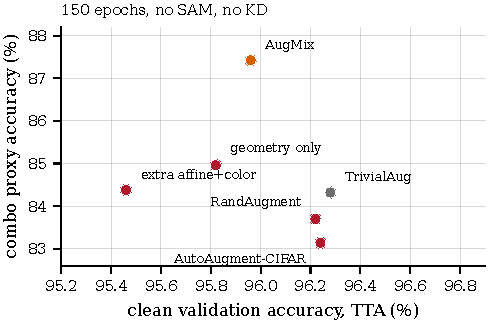
\includegraphics[width=\columnwidth]{figures/fig_b3_pilot.pdf}
\caption{Augmentation pilot at 150 epochs (no SAM, no KD). Each point is one
policy; the vertical axis is the composite corruption proxy. One-view AugMix is
the only policy that is clean-neutral and improves the proxy. The pilot
overstates the effect because the 300-epoch control is stronger.}
\label{fig:b3}
\end{figure}

\paragraph{The 300-epoch test.}
At 300 epochs with SAM, AugMix and the TrivialAugment control are identical on
clean validation (EMA 97.08\% both; flip TTA 97.04 vs.\ 97.22;
Figure~\ref{fig:robustness}). Under the no-TTA shifted evaluation, AugMix
improves the composite by 2.18 points (89.02 vs.\ 86.84, McNemar
$p=3.6\times10^{-9}$), Gaussian noise 0.05 by 4.30, and JPEG-30 by 5.16. Under
flip TTA it improves mild and strong photographic jitter by 1.10 and 1.38 points
($p\approx10^{-5}$). Geometry alone is where AugMix does nothing (+0.06 on
$\pm3$-pixel shifts), which is consistent with the gain coming from photometric
variation rather than framing. A second AugMix seed reproduces the effect (+1.80
composite; mean +1.99 across seeds) and keeps clean accuracy neutral (96.90\%).

\paragraph{Distillation.}
The provisional KD check uses the same \texttt{r3\_80} student, three teachers,
and 300 epochs, changing only \texttt{--autoaug}. In the checkpoint comparison at
epoch 200 of 300 (the archived logs stop earlier), AugMix is clean-neutral
($-0.12$, $p=0.56$) and better on the composite (+2.20,
$p=3.7\times10^{-12}$) and strong photographic jitter (+1.92,
$p=5.6\times10^{-12}$); the geometry proxy moves by +0.36 ($p=0.069$). At that
point the AugMix arm is level with the 600-epoch A4 model on the composite
(89.26 vs.\ 89.20) while still about one point behind on clean (96.86 vs.\
97.84). The effect therefore provisionally survives distillation at roughly the
same size as in the no-KD comparison. The run was interrupted and the two logs
stop at epochs 163 and 178 of 300; the comparison is provisional and was not used
for submission selection.

\paragraph{The JSD caveat.}
The B4/B5 variant is image-only, one-view AugMix without the Jensen-Shannon
consistency term. A separate 80-epoch AugMix+JSD finisher (JSD weight 12, ramped
over 10 epochs) behaved differently: it gained 2.2 points on the blur proxy
relative to the matched control but lost about one point on clean validation
(96.88 vs.\ 97.44 for the control and 97.84 for untouched A4). It failed our
clean-accuracy gate and was not submitted. The clean-neutral result should
therefore be read as specific to the one-view variant at the schedules we tested,
not to AugMix with JSD.

\begin{figure*}[t]
\centering
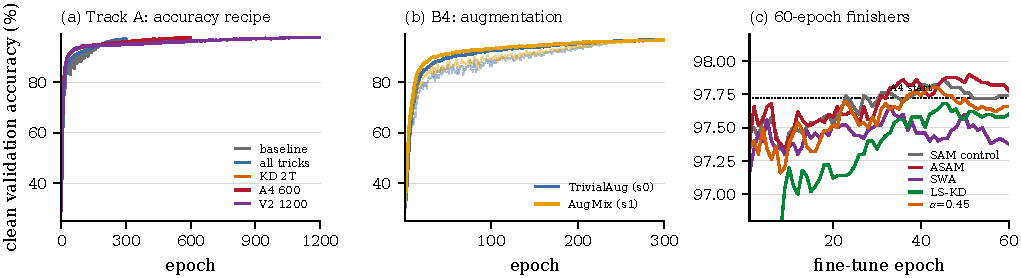
\includegraphics[width=\textwidth]{figures/fig_val_curves.pdf}
\caption{Validation curves (EMA weights unless noted, no TTA). (a) Main recipe:
baseline (raw), all tricks, two-teacher KD, A4 (600 epochs), and V2 (1,200
epochs). (b) Architecture sweep at 300 epochs. (c) KD-temperature/weight sweep;
the two logs stop at epochs 181 and 183 of 300. (d) 60-epoch continuations from
A4; the dotted line is the untouched A4 EMA on the same no-TTA evaluation
(97.72). The finishers stay within 0.35 points of it; none is a significant
gain. (e) Fresh 300-epoch alternatives: the WRN-40-2 pair, LS-KD, and fresh
ASAM; late training is shown and none beats the 97.66\% control. (f) The
provisional KD + AugMix arms; logs stop at epochs 163 and 178 of 300. Final
flip/5-crop TTA numbers are in Tables~\ref{tab:main} and~\ref{tab:negative}.}
\label{fig:curves}
\end{figure*}

\begin{figure*}[t]
\centering
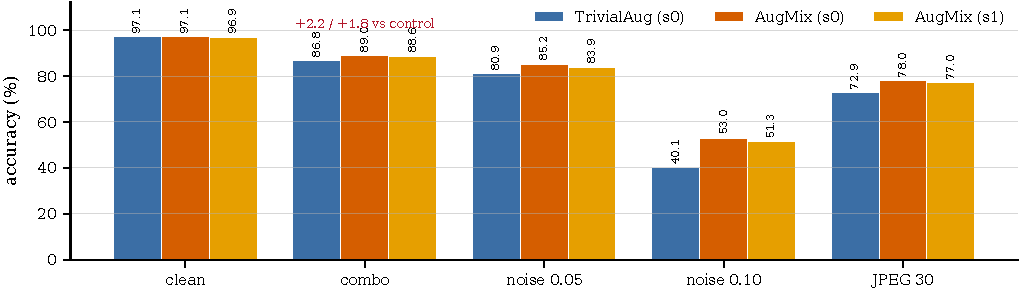
\includegraphics[width=\textwidth]{figures/fig_robustness.pdf}
\caption{Clean and shifted accuracy for the 300-epoch B4 arms (EMA weights, no
TTA). One-view AugMix is clean-neutral and improves the composite, noise, and
JPEG proxies; the two seeds give +2.18 and +1.80 on the composite. These are
label-free stress tests built from training images.}
\label{fig:robustness}
\end{figure*}

\subsection{Test-Time Augmentation}

Flip TTA is the default. The 10-view 5-crop procedure adds essentially nothing
on clean data (trivial $-0.02$, AugMix $+0.10$) and is a wash overall
(Figure~\ref{fig:tta}): it helps on JPEG and the composite by 0.5--1.2 points, but
loses on noise and zoom. It costs ten times the inference. We nevertheless used
5-crop for the 0.911 submission because it exactly reproduced the team's accepted
CSV; the gain over flip is inside leaderboard noise and should not be attributed
to TTA.

\begin{figure}[t]
\centering
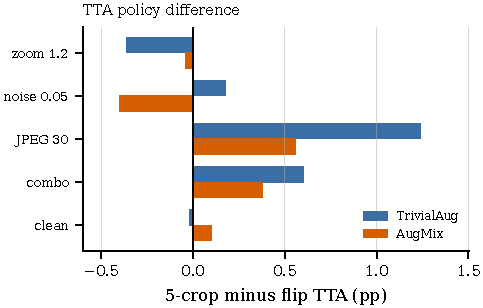
\includegraphics[width=\columnwidth]{figures/fig_tta_deltas.pdf}
\caption{5-crop minus flip TTA on the B4 arms. The multi-view policy helps on
JPEG and the composite, is negligible on clean data, and hurts on noise and zoom;
the 10$\times$ inference cost is not justified by the clean result.}
\label{fig:tta}
\end{figure}

\subsection{The Leaderboard}

Figure~\ref{fig:leaderboard} shows every public submission. The selected
\texttt{F2s1} 5-crop run is the best at 0.911; the two-teacher student is 0.904.
Late finishers and soups built on \texttt{F2s1} score 0.908, below the untouched
model, and test-time BN adaptation drops to 0.884. The private score is 0.880 and
the team finished 13th. The gap between the 97.94\% holdout and the 0.880 private
score is the central unexplained result: we do not have the final evaluation
labels or images, so we cannot identify whether it comes from a different capture
distribution, a harder class mix, or a smaller effective test set. We report it
as observed and do not tune against it.

\begin{figure}[t]
\centering
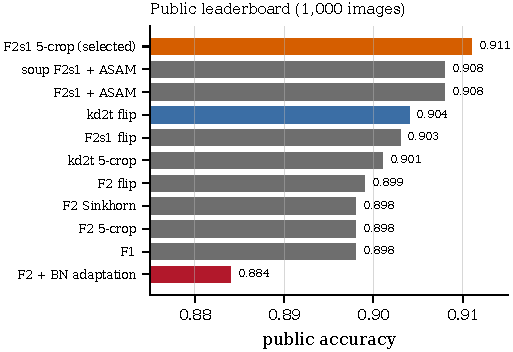
\includegraphics[width=\columnwidth]{figures/fig_leaderboard.pdf}
\caption{All public leaderboard submissions (1,000 images). The selected
\texttt{F2s1} 5-crop model is the best at 0.911; late ASAM/soup finishers sit at
0.908 and test-time BN adaptation at 0.884. Public scores carry roughly
$\pm1.1$pp of noise, so differences of a few images are not a model ranking.}
\label{fig:leaderboard}
\end{figure}
